Lung cancer is a disease characterized by the uncontrolled growth of abnormal cells in the tissues of the lungs. These abnormal cells can form tumors that interfere with the normal functioning of the lungs, such as breathing and oxygen exchange. Lung cancer is one of the leading causes of cancer-related deaths worldwide due to its high prevalence and often late-stage diagnosis.

\section{How does Lung Cancer develop?}
\begin{remark}
Lung cancer \cite{li2024gut} typically begins in the cells lining the airways. These cells undergo genetic mutations that cause them to grow uncontrollably and lose their normal function. Over time, these cells can invade surrounding tissues and spread to other parts of the body, a process known as metastasis \cite{shi2024mechanism}.
\end{remark}

\section{Global Impact}
\begin{outline}
Lung cancer has a significant global impact \cite{ramamoorthy2024assessing}, with millions of new cases and deaths reported annually. It is more common in regions with high smoking rates and industrial exposure. Early detection and preventive measures such as smoking cessation programs can greatly reduce the burden of this disease.
\end{outline}

\begin{figure}[h!]
    \centering
    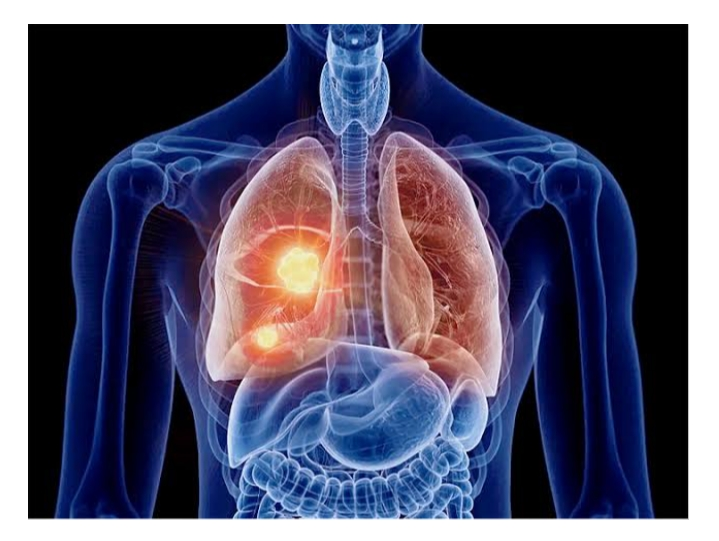
\includegraphics[width= 0.85\linewidth]{images/lung_c.jpeg}
    \caption{Lung cancer}
    \label{fig:enter-label}
\end{figure}